% -*- coding: UTF-8 -*-
% vim: autoindent expandtab tabstop=4 sw=4 sts=4 filetype=tex
% vim: spelllang=de spell
% chktex-file 27 - disable warning about missing include files

\chapter{Prototyp}
\label{chap:prototype}

Nach dem Finden und Ausarbeiten der Vision
(siehe~\autoref{subsec:requirements:vision}) sowie der Identifikation der
wichtigsten Komponenten (siehe~\autoref{sec:main-components}), wurde ein
Prototyp von Teilen der geplanten Software umgesetzt. Dies diente auch der
Identifikation der zusätzlichen Anforderungen
(siehe~\autoref{subsec:requirements:additional-requirements}).

Der Prototyp erlaubt die Modellierung einer einfachen Szene, bestehend aus
Primitiven, anhand der Graph-Komponente. Die Primitiven befinden sich in
externen (Shader-) Dateien, welche zur Laufzeit zusammen mit einem Haupt-Shader
geladen und zur Verfügung gestellt werden. Die nachfolgende Auflistung zeigt
die möglichen Unterverzeichnisse und Datei-Typen.

\begin{itemize}
    \item \textbf{data/objects/*.fs.xml}\\
        Sämtliche Objekt-Definitionen, wie zum Beispiel Kugel oder Würfel.
    \item \textbf{data/operations/*.fs.xml}\\
        Sämtliche Operationen, wie zum Beispiel die Vereinigung von Objekten.
    \item \textbf{data/misc/*.fs.xml}\\
        Diverse andere Definitionen, wie zum Beispiel Kameras.
    \item \textbf{data/sphere\_tracer.fs}\\
        Die Haupt-Shader-Datei, welche um Objekte, Operationen oder andere
        Definitionen ergänzt wird.
\end{itemize}

Durch die Modellierung wird der Haupt-Shader um Teile ergänzt und neu kompiliert, dies geschieht alles zur
Laufzeit in Echtzeit. Die Darstellung findet schliesslich mittels dem als
Sphere-Tracing bekannten Ray-Tracing-Verfahren
statt.~\autoref{listing:prototype:objects:sphere}
und~\autoref{listing:prototype:operations:union} zeigen Beispiel von
Shader-Defintionen.

\begin{minipage}{\linewidth}
\begin{lstlisting}[language=XML,caption={Objekt-Definition einer Kugel
        in XML.},label={listing:prototype:objects:sphere},captionpos=b,emph={xmlns,version,type}]
<?xml version="1.0" encoding="UTF-8"?>
<function>
    <name>sphere</name>
    <return-type>float</return-type>
    <parameters>
        <parameter>
            <name>position</name>
            <builtin>vec3</builtin>
            <type>property</type>
            <call>position - {}</call>
        </parameter>
        <parameter>
            <name>radius</name>
            <builtin>float</builtin>
            <type>property</type>
            <call>{}</call>
        </parameter>
    </parameters>
    <source>
        // Returns the signed distance to a sphere with given radius for the
        // given position.
        float sphere(vec3 position, float radius)
        {
            return length(position) - radius;
        }
    </source>
</function>
\end{lstlisting}
\end{minipage}

\begin{minipage}{\linewidth}
\begin{lstlisting}[language=XML,caption={Definition des Vereinigungs-Operators
        in XML.},label={listing:prototype:operations:union},captionpos=b,emph={castRay}]
<?xml version="1.0" encoding="UTF-8"?>
<function>
    <name>opUnion</name>
    <return-type>float</return-type>
    <parameters>
        <parameter>
            <name>a</name>
            <builtin>float</builtin>
            <type>input</type>
            <call>{}</call>
        </parameter>
        <parameter>
            <name>b</name>
            <builtin>float</builtin>
            <type>input</type>
            <call>{}</call>
        </parameter>
    </parameters>
    <source>
        // Returns the signed distance for a merge of given signed
        // distance a and signed distance b.
        float opUnion(float a, float b)
        {
            return min(a, b);
        }
    </source>
</function>
\end{lstlisting}
\end{minipage}

% -*- coding: UTF-8 -*-
% vim: autoindent expandtab tabstop=4 sw=4 sts=4 filetype=tex
% vim: spelllang=de spell
% chktex-file 27 - disable warning about missing include files

\section{Vorgehen}
\label{sec:prototype:procedure}

Die Entwicklung des Prototypen war ein iterativer Prozess. Es wurden Teil-Ziele
definiert, welche dann etappenweise erarbeitet wurden.

Das erste Teil-Ziel war das Neu-Kompilieren von Shadern während der Laufzeit,
so dass Shader während der Laufzeit erweitert, neu geladen und dargestellt
werden können.

Als zweites Teil-Ziel wurde dynamisches Laden von Shader-Dateien ausgehend vom
Verzeichnis des Prototypen implementiert.

Als drittes Teil-Ziel wurden Shader in Form von Templates umgesetzt.  Mit
``Jinja2CppLight'' (TODO~\todo{add reference to Jinja2CppLight here}) wurde
schliesslich ein Template-System eingeführt, welches es erlaubt Shader als
Templates zu parsen und Sektionen entsprechend mit Sub-Templates respektive
Teil-Shadern zu ersetzen.  Dies ermöglicht es Teile von Shadern während der
Laufzeit anzupassen. Durch die Erkenntnisse des ersten Teil-Zieles konnte der
aus dem Template zusammen mit den Sub-Templates generierte Shader zur Laufzeit
geladen und ausgeführt werden.

Als viertes und letztes Teil-Ziel wurde ein Prototyp der Graph-Komponente
(siehe~\ref{ssubsec:main-components:editor:graph}) umgesetzt. Der Graph bietet
ein Kontext-Menü zum Hinzufügen und Entfernen von Knoten. Für jeden
eingelesenen Teil-Shader wird ein Eintrag im Kontext-Menü hinzugefügt, so dass
dieser schliesslich dem Graphen hinzugefügt werden kann. Der Graph verfügt
standardmässig immer über einen (Haupt-) Ausgangs-Knoten.

Jeder der Knoten verfügt entweder über mindestens einen Eingang oder über einen
Ausgang.  Zusätzliche Ein- beziehungsweise Ausgänge werden je nach Typ eines
Knotens automatisch, dynamisch erstellt. Die Eingänge des Haupt-Knotens sind
jedoch statisch. Dieser verfügt über eine Haupt-Schnittstelle sowie eine
Schnittstelle für einen Kamera-Knoten.

Bei jeder neuen Verbindung beziehungsweise bei jedem Trennen einer Verbindung
innerhalb des Graphen, wird dieser neu evaluiert und die (Shader-) Ausgabe neu
berechnet.

Das Rendering ist schliesslich die Berechnung der relevanten Matrizen, binden
des Shaders und setzen der benötigten Uniform-Variablen.
Abbildung~\ref{fig:prototype:procedure} zeigt den aktuellen Stand des
Prototypen.

\begin{figure}[H]
    \centering
    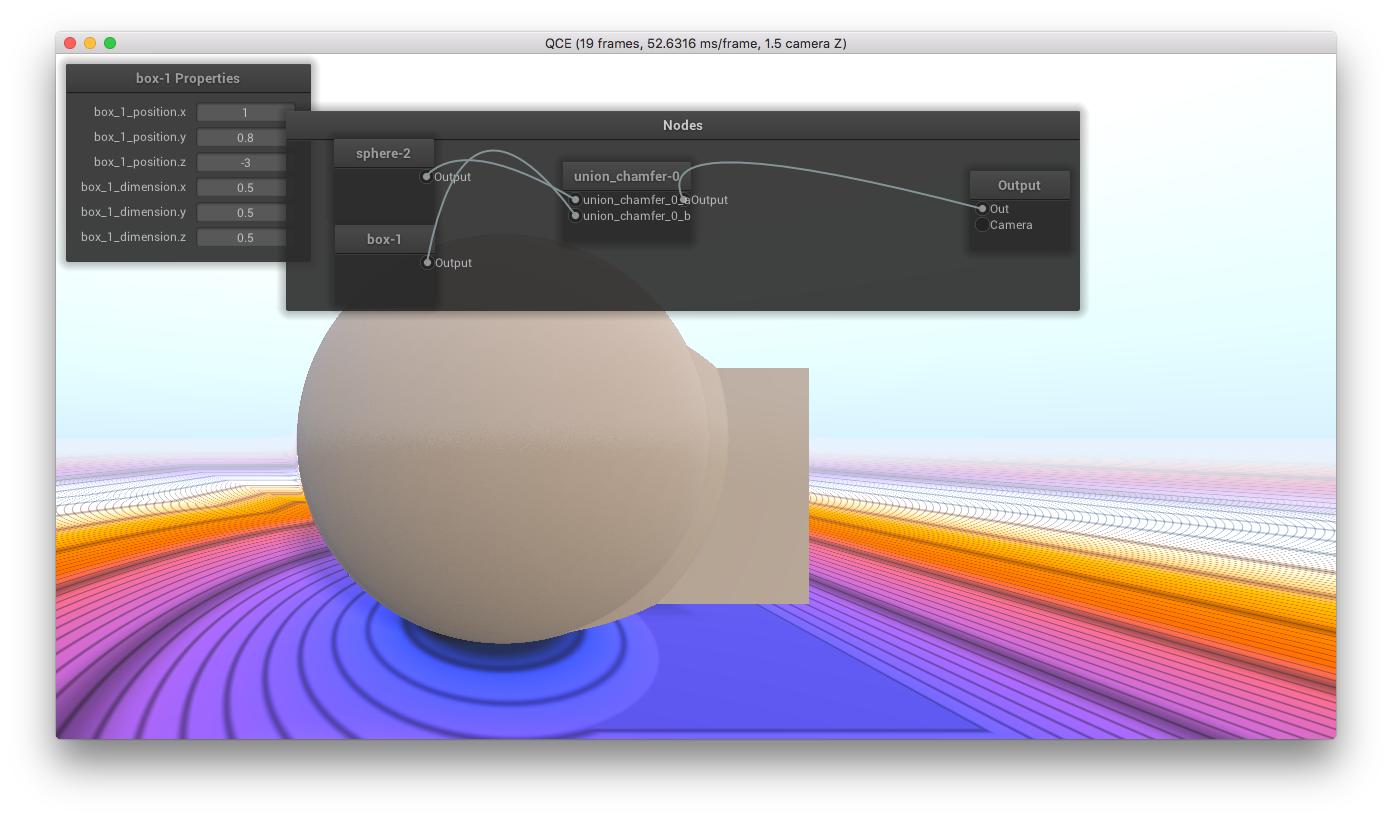
\includegraphics[width=0.9\textwidth]{img/prototype.png}
    \caption{Der Prototyp in Aktion
        \protect\footnotemark}\label{fig:prototype:procedure}
\end{figure}
\footnotetext{Eigene Darstellung.}

% -*- coding: UTF-8 -*-
% vim: autoindent expandtab tabstop=4 sw=4 sts=4 filetype=tex
% vim: spelllang=de spell
% chktex-file 27 - disable warning about missing include files

\section{Domänenmodell und Klassendiagramm}
\label{sec:prototype:domain-model-class-diagram}

Für den Prototypen wurde nicht explizit ein Domänenmdodell festgehalten. Dieses
wurde anhand der Vision und der Komponenten erstellt. Überlegungen dazu flossen
direkt in das Domänenmodell der Software-Architektur ein
(siehe~\autoref{sec:domain-model}).

In Abbildung~\ref{fig:class-diagram:prototype} findet sich das Klassendiagramm
des Prototypen. Blau-graue Elemente stellen dabei selbst entwickelte Pakete,
violette Elemente externe Pakete von Drittpersonen dar. Es wird bewusst
nicht das vollständige Klassendiagramm mit allen Elementen abgebildet, da dies
nach Meinung des Autors zu unübersichtlich würde. Die gesamte Struktur ist dem
Programmcode des Prototypen zu entnehmen, welcher dieser Projektarbeit
beiliegt.

\begin{figure}[H]
    \centering
    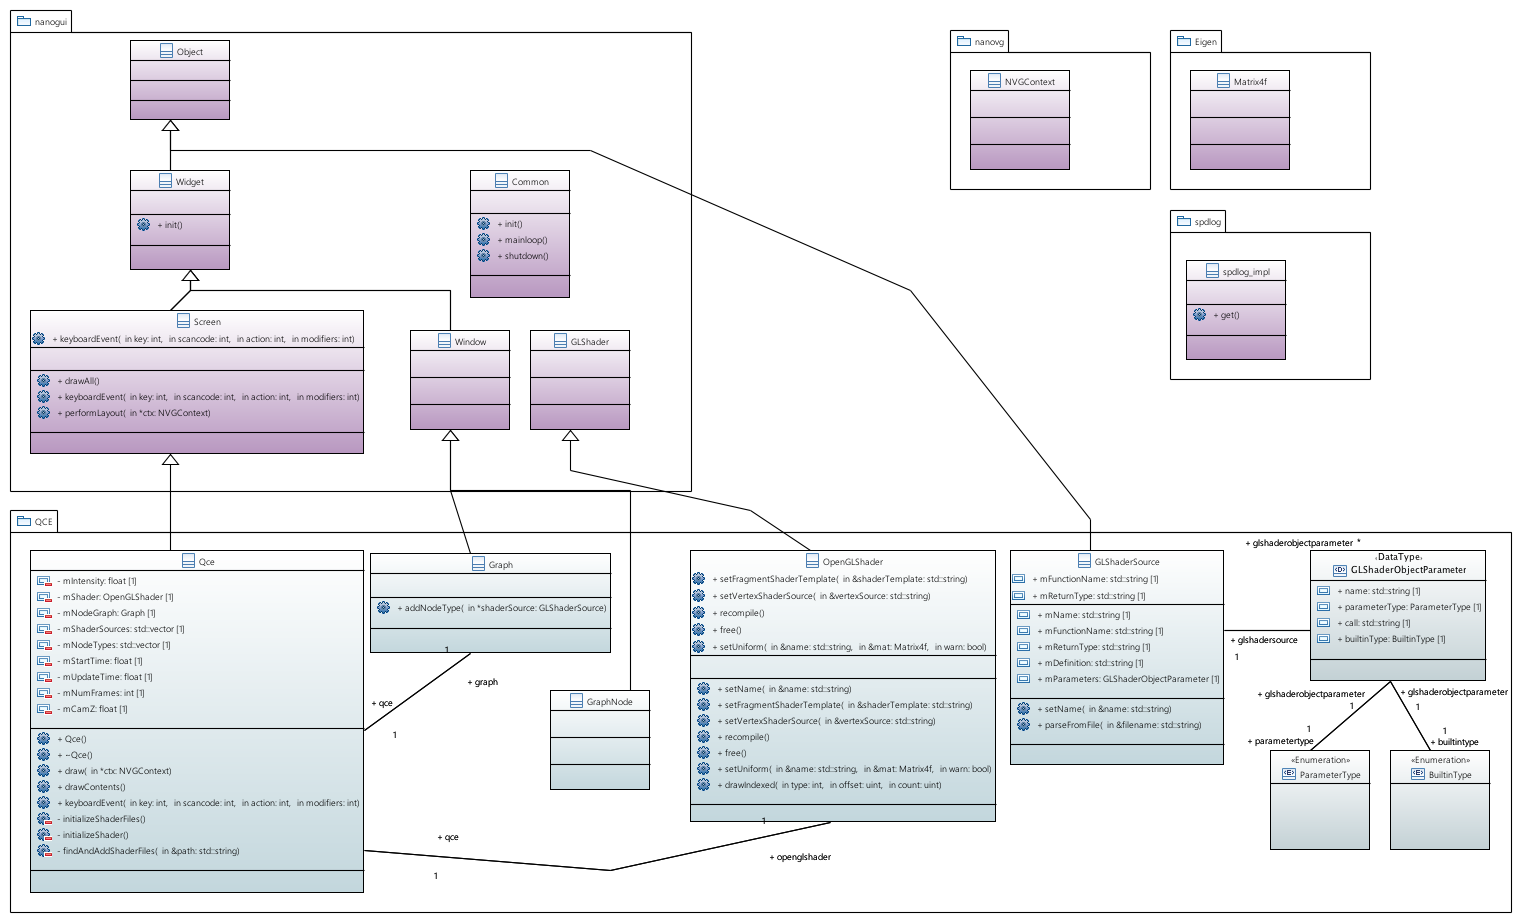
\includegraphics[angle=90,width=0.9\textwidth]{img/prototype_class_diagram.png}
    \caption{Klassendiagramm der Prototyp-Applikation}\label{fig:class-diagram:prototype}
\end{figure}

% -*- coding: UTF-8 -*-
% vim: autoindent expandtab tabstop=4 sw=4 sts=4 filetype=tex
% vim: spelllang=de spell
% chktex-file 27 - disable warning about missing include files

\section{Programmablauf}
\label{sec:prototype:sequence}

Nach dem Starten der Applikation erstellt diese die grafische
Benutzeroberfläche und lädt alle externen Shader-Dateien im Unterverzeichnis 
``data''. Die Haupt-Shader-Datei wird als Grundlage für den Ausgabe-Shader
genutzt, die Teil-Shader-Dateien bilden die wählbaren Objekte beziehungsweise
Einträge im Kontextmenü des Graphen.

Nach dem initialen Berechnen und Darstellen der Benutzeroberfläche befindet
sich die Applikation schliesslich in der Hauptschleife. Die Hauptschleife läuft
so lange bis der Benutzer diese mittels Tastendruck auf die Escape-Taste
unterbricht und damit die Applikation beendet.

In der Hauptschleife verarbeitet die Applikation diverse Events wie zum
Beispiel Maus- und Tastatur-Eingaben. Die Verarbeitung findet in der Regel
zuerst in den Kind-Klassen und dann schliesslich in der Hauptklasse statt. Dies
erlaubt es diversen Komponenten, welche eben Kind-Klassen der Applikation sind,
auf Ereignisse, wie zum Beispiel dem Erstellen einer Verbindung zwischen zwei
Knoten, zu reagieren.

Immer wenn ein Knoten dem Haupt-Ausgabeknoten des Graphen direkt oder indirekt
hinzugefügt wird, wird der Graph und somit der Shader neu berechnet
beziehungsweise kompiliert.

Beendet der Benutzer schliesslich die Hauptschleife via Druck auf die
Escape-Taste, so werden alle Ressourcen frei gegeben und die Applikation wird
beendet.

Eine vereinfachte Darstellung des Beschriebenen findet sich in
Abbildung~\ref{fig:prototype:sequence:activity}. Eine detailliertere
Darstellung findet sich in Abbildung~\ref{fig:prototype:sequence:diagram}.

\begin{figure}[H]
    \centering
    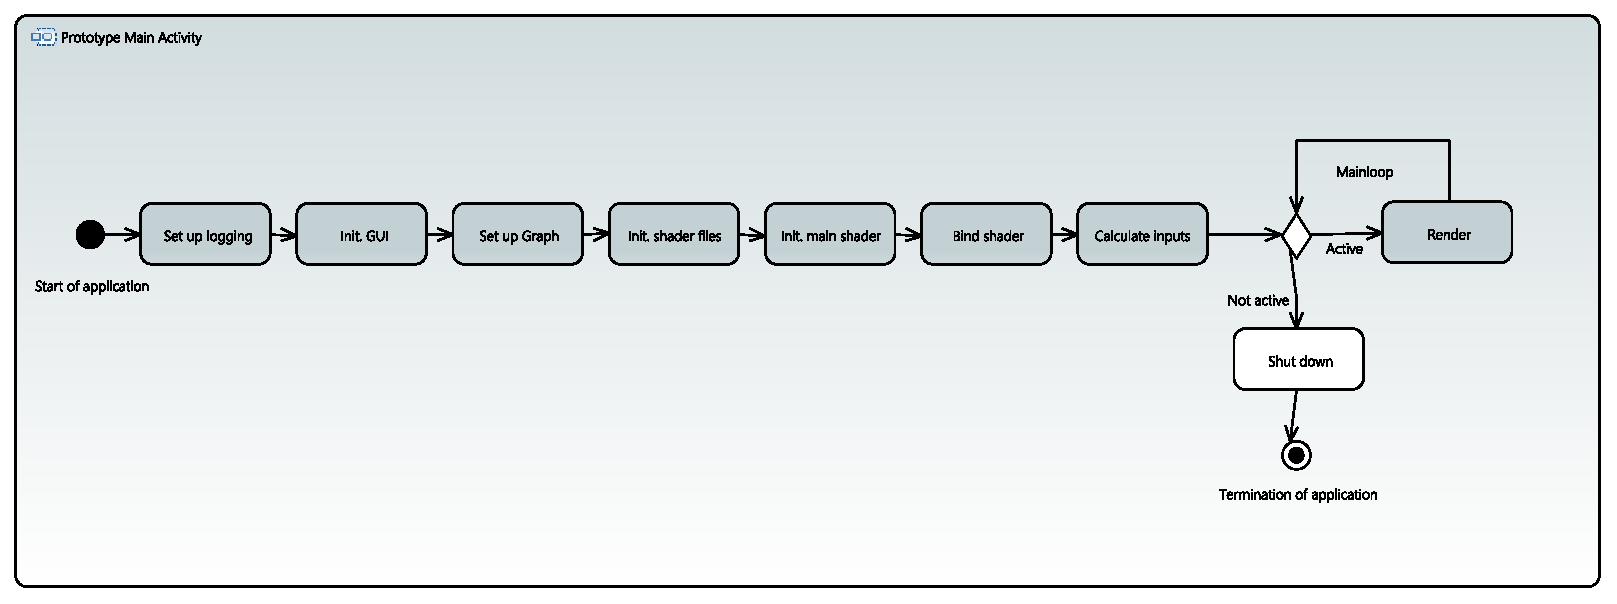
\includegraphics[width=0.9\textwidth]{img/prototype_activity_diagram.png}
    \caption{Vereinfachte Darstellung des Haupt-Programmablaufes
        \protect\footnotemark}\label{fig:prototype:sequence:activity}
\end{figure}
\footnotetext{Eigene Darstellung mittels Papyrus.}

\begin{figure}[H]
    \centering
    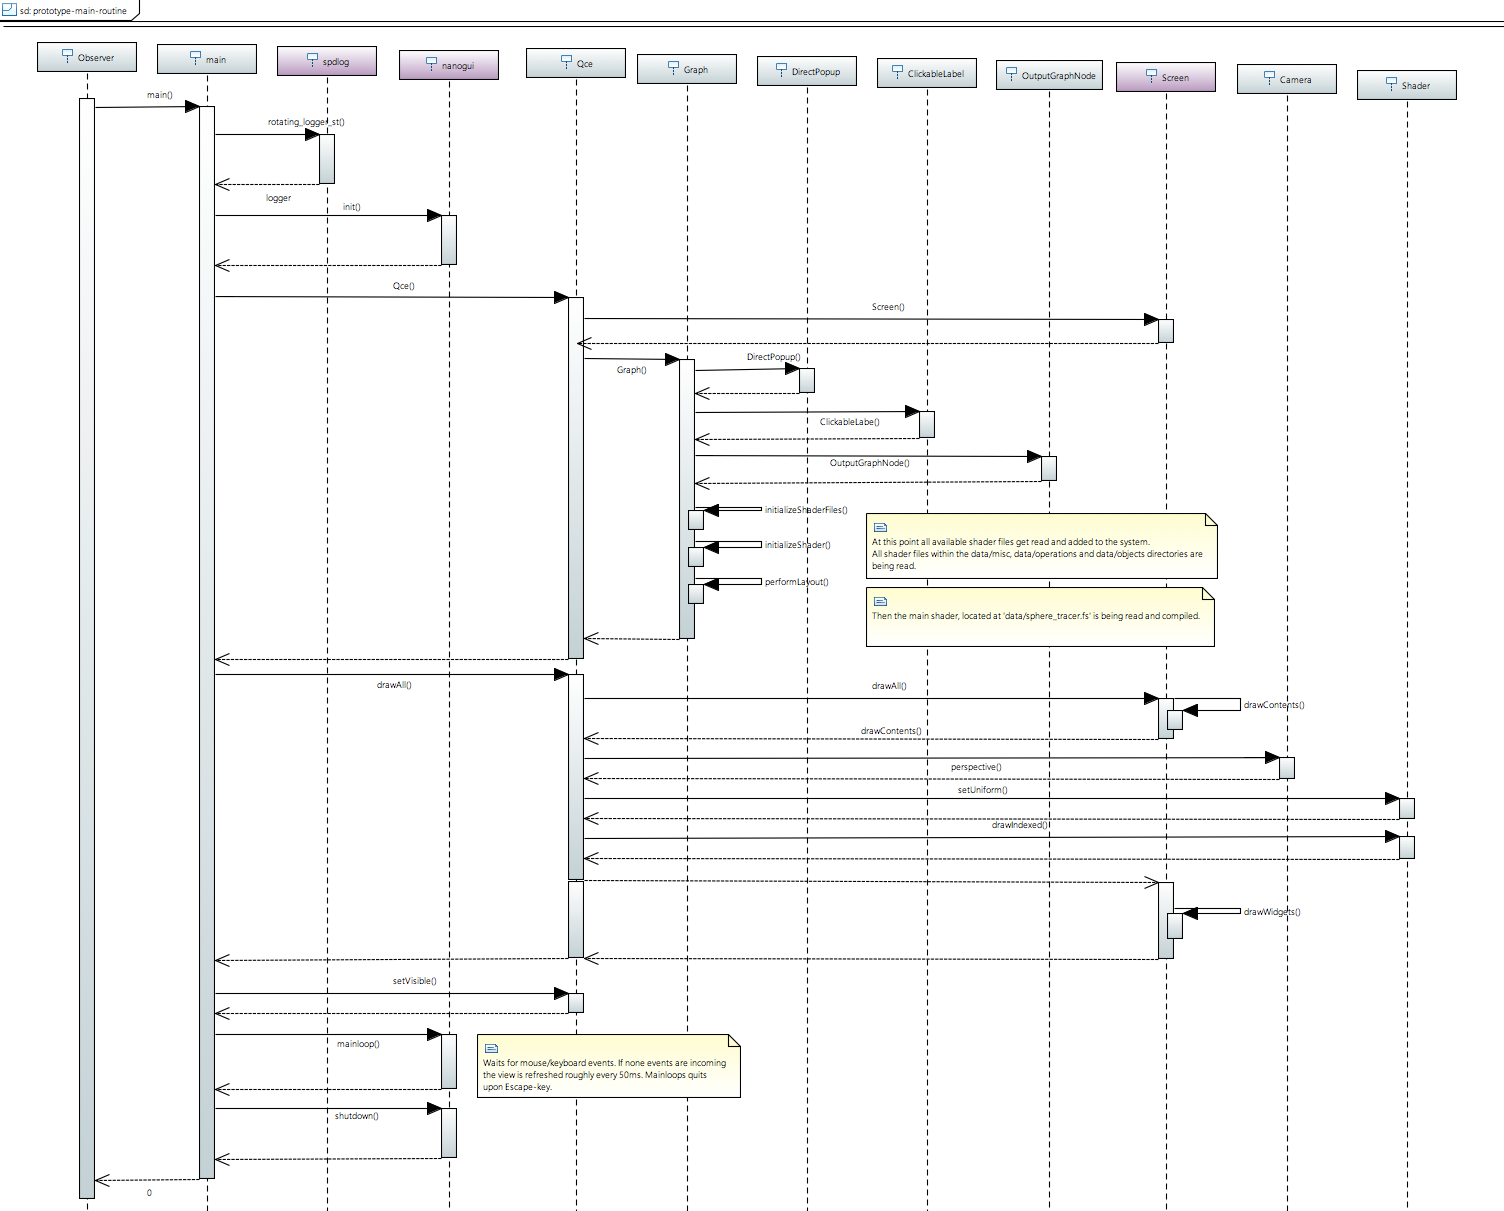
\includegraphics[width=0.9\textwidth]{img/prototype_sequence_diagram.png}
    \caption{Sequenz-Diagramm des Haupt-Ablaufes der
        Prototyp-Applikation\protect\footnotemark}\label{fig:prototype:sequence:diagram}
\end{figure}
\footnotetext{Eigene Darstellung mittels Papyrus.}

% -*- coding: UTF-8 -*-
% vim: autoindent expandtab tabstop=4 sw=4 sts=4 filetype=tex
% vim: spelllang=de spell
% chktex-file 27 - disable warning about missing include files

\section{Komponenten}
\label{sec:main-components}

Ausgehend von den Anforderungen (\ref{sec:requirements}) können einzelne
Komponenten der Applikation abgeleitet werden. Einzelne Teile davon wurden
schon durch die Vision (\ref{sec:vision}) definiert beziehungsweise aus dieser
gewonnen.

Dieser Prozess entspricht nicht direkt dem Vorgehen
gemäss~\cite{larman_applying_2004} beziehungsweise dem UP, der Autor dieser
Projektarbeit ist jedoch der Ansicht, dass dieser Abschnitt eine Brücke
zwischen Anforderungen und der (Software-) Modellierung bildet. Zudem bietet
dieser Abschnitt eine relativ bildliche Beschreibung, was dem Verständnis des
Gesamtkonzeptes sicher zuträglich ist. Am ehesten entspricht dieser Abschnitt
den Komponenten-Diagrammen in~\cite[S. 653 bis 654]{larman_applying_2004}.

Die Applikation besteht aus zwei Applikationen: Einem \textit{Player},
welcher dem Abspielen von Echtzeit-Animationen dient, sowie einem \textit{Editor},
welcher der Erstellung und Verwaltung von Echtzeit-Animationen dient.

\subsection{Player}
\label{subsec:main-components:player}

Der \textit{Player} liest die vom \textit{Editor} exportierten
Echtzeit-Animationen. Er bietet vor dem Abspielen die Auswahl der Auflösung,
des Seitenverhältnisses, Antialiasing und ob die Animation im Vollbild-Modus
abgespielt werden soll.

\subsection{Editor}
\label{subsec:main-components:editor}

Der \textit{Editor} erlaubt das Erstellen und Bearbeiten von
Echtzeit-Animationen. Diese können schliesslich inklusive den
dazugehörigen Dateien, wie zum Beispiel Bitmaps oder Modellen, exportiert
werden.

\begin{figure}[h]
    \centering
    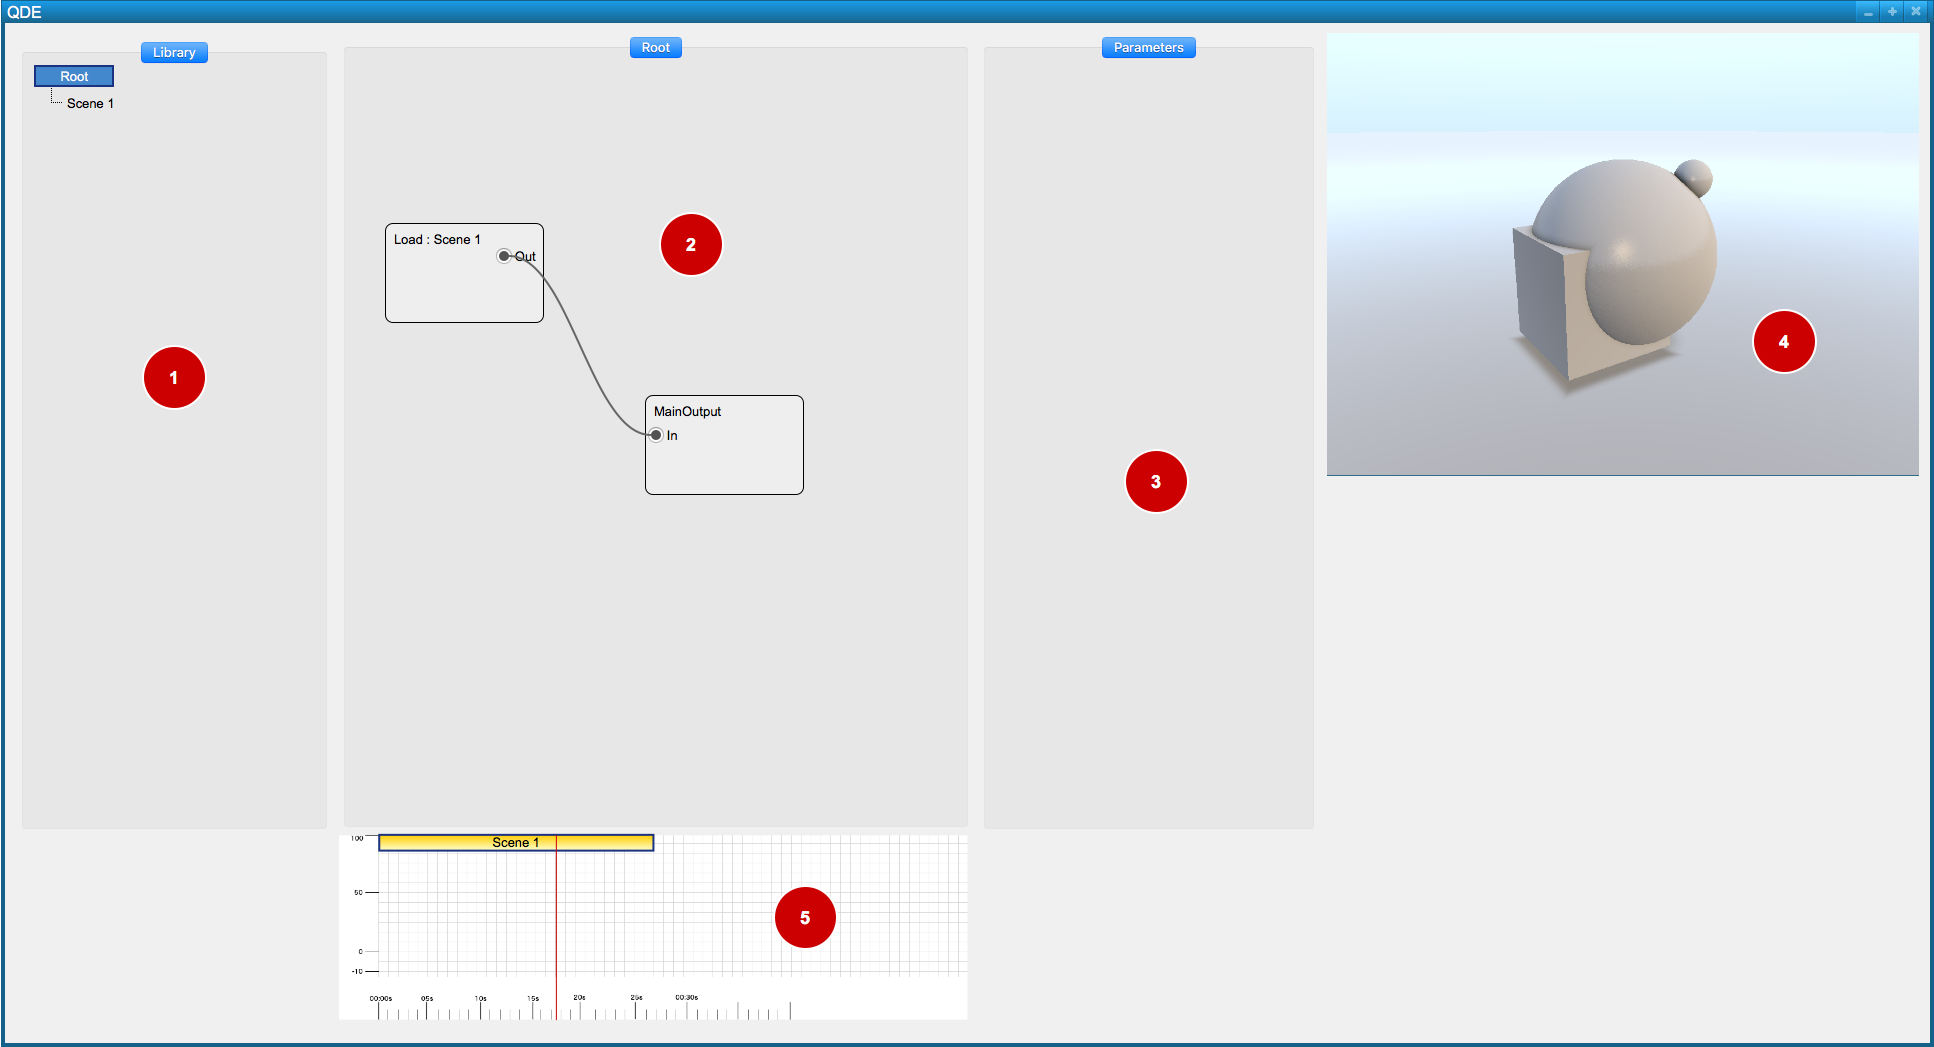
\includegraphics[width=0.9\textwidth]{img/editor_components.png}
    \caption{Einzelne Komponenten des Editors
        \protect\footnotemark}\label{fig:main-components:editor:editor-components}
\end{figure}
\footnotetext{Eigene Darstellung mittels Pencil.}

Abbildung~\ref{fig:main-components:editor:editor-components} zeigt die
einzelnen Komponenten des Editors. Nachfolgend findet sich eine Beschreibung
dieser.

\subsubsection{Bibliothek}
\label{ssubsec:main-components:editor:library}

Das Element~\img{img/editor_component_1.png} in
Abbildung~\ref{fig:main-components:editor:editor-components} zeigt die (Szenen-)
Bibliothek. Diese beinhaltet alle Szenen einer Echtzeit-Animation. Es können
neue Szenen angelegt und auch bestehende Szenen gelöscht werden. Wird ein neues
Projekt erstellt, so verfügt dieses immer über die ``Root''-Szene. Diese
beinhaltet den Haupt-Ausgabeknoten des Graphen
(\ref{ssubsec:main-components:editor:graph}), welcher schliesslich zum
Abspielen evaluiert wird, und kann nicht gelöscht werden. Wird eine Szene mit
der Maus angewählt, so wird deren Inhalt im Graphen
(\ref{ssubsec:main-components:editor:graph}) dargestellt.

\subsubsection{Graph}
\label{ssubsec:main-components:editor:graph}

Das Element~\img{img/editor_component_2.png} in
Abbildung~\ref{fig:main-components:editor:editor-components} zeigt den Graphen
einer Szene. Dieser beinhaltet sämtliche Knoten einer Szene. Mittels
Kontextmenü können neue Knoten eingefügt und bestehende Knoten gelöscht werden.
Wird ein Knoten angewählt, so wird dieser einerseits im
Rendering-Ansichtsfenster (\ref{ssubsec:main-components:editor:rendering})
dargestellt, andererseits werden dessen Eigenschaften im Parameter-Fenster
(\ref{ssubsec:main-components:editor:parameters}) angezeigt.

Folgende Typen von Knoten sind geplant:
\begin{itemize}
    \item{Scene}
    \item{TimelineClip}
    \item{Model}
    \item{Camera}
    \item{Light}
    \item{Material}
    \item{Operator}
    \item{Effect}
\end{itemize}

\subsubsection{Parameter}
\label{ssubsec:main-components:editor:parameters}

Das Element~\img{img/editor_component_3.png} in
Abbildung~\ref{fig:main-components:editor:editor-components} zeigt die Parameter
des aktuell gewählten Knoten im Graphen
(\ref{ssubsec:main-components:editor:graph}). Neben jedem Parameter befindet
sich eine Schaltfläche zum Setzen von Schlüsselbildern (Keyframes) in der
Zeitachse (Timeline,~\ref{ssubsec:main-components:editor:timeline}). Wird die
Schaltfläche betätigt, so wird bei dem aktuell ausgewählten Zeitpunkt der
Zeitachse ein Schlüsselbild gesetzt.

\subsubsection{Rendering}
\label{ssubsec:main-components:editor:rendering}

Das Element~\img{img/editor_component_4.png} in
Abbildung~\ref{fig:main-components:editor:editor-components} zeigt das
Rendering-Ansichtsfenster. Dieses stellt den Inhalt des aktuell gewählten
Knotens dar. Die Art des Knotens ist dabei nicht beschränkt, es kann dies eine
Szene, aber zum Beispiel auch ein einzelnes Modell sein. Es wird immer der
gesamte vorhergehende (Teil-) Baum des Knotens evaluiert.

\subsubsection{Zeitachse}
\label{ssubsec:main-components:editor:timeline}

Die Zeitachse wird mit~\img{img/editor_component_5.png} in
Abbildung~\ref{fig:main-components:editor:editor-scene1} dargestellt.  Sie
bildet das zeitliche Geschehen einer Echtzeit-Animation ab. Alle Knoten vom Typ
Timeline-Clip werden am oberen Rand des Fensters in deren zeitlicher
Reihenfolge abgebildet. Wird im Graph
(\ref{ssubsec:main-components:editor:graph}) ein Knoten mit animierten
Parametern (\ref{ssubsec:main-components:editor:parameters}) angewählt, so sind
diese ersichtlich. Vertikal wird der Wertebereich, horizontal die Zeitachse in
Sekunden dargestellt. Ein vertikal verlaufender, roter Marker zeigt die aktuelle
zeitliche Position der Echtzeit-Animation an.

Die untenstehende Abbildung~\ref{fig:main-components:editor:editor-scene1} zeigt ein Beispiel, wie eine typische Szene
mit animierten Parametern aussehen könnte.

\begin{figure}[H]
    \centering
    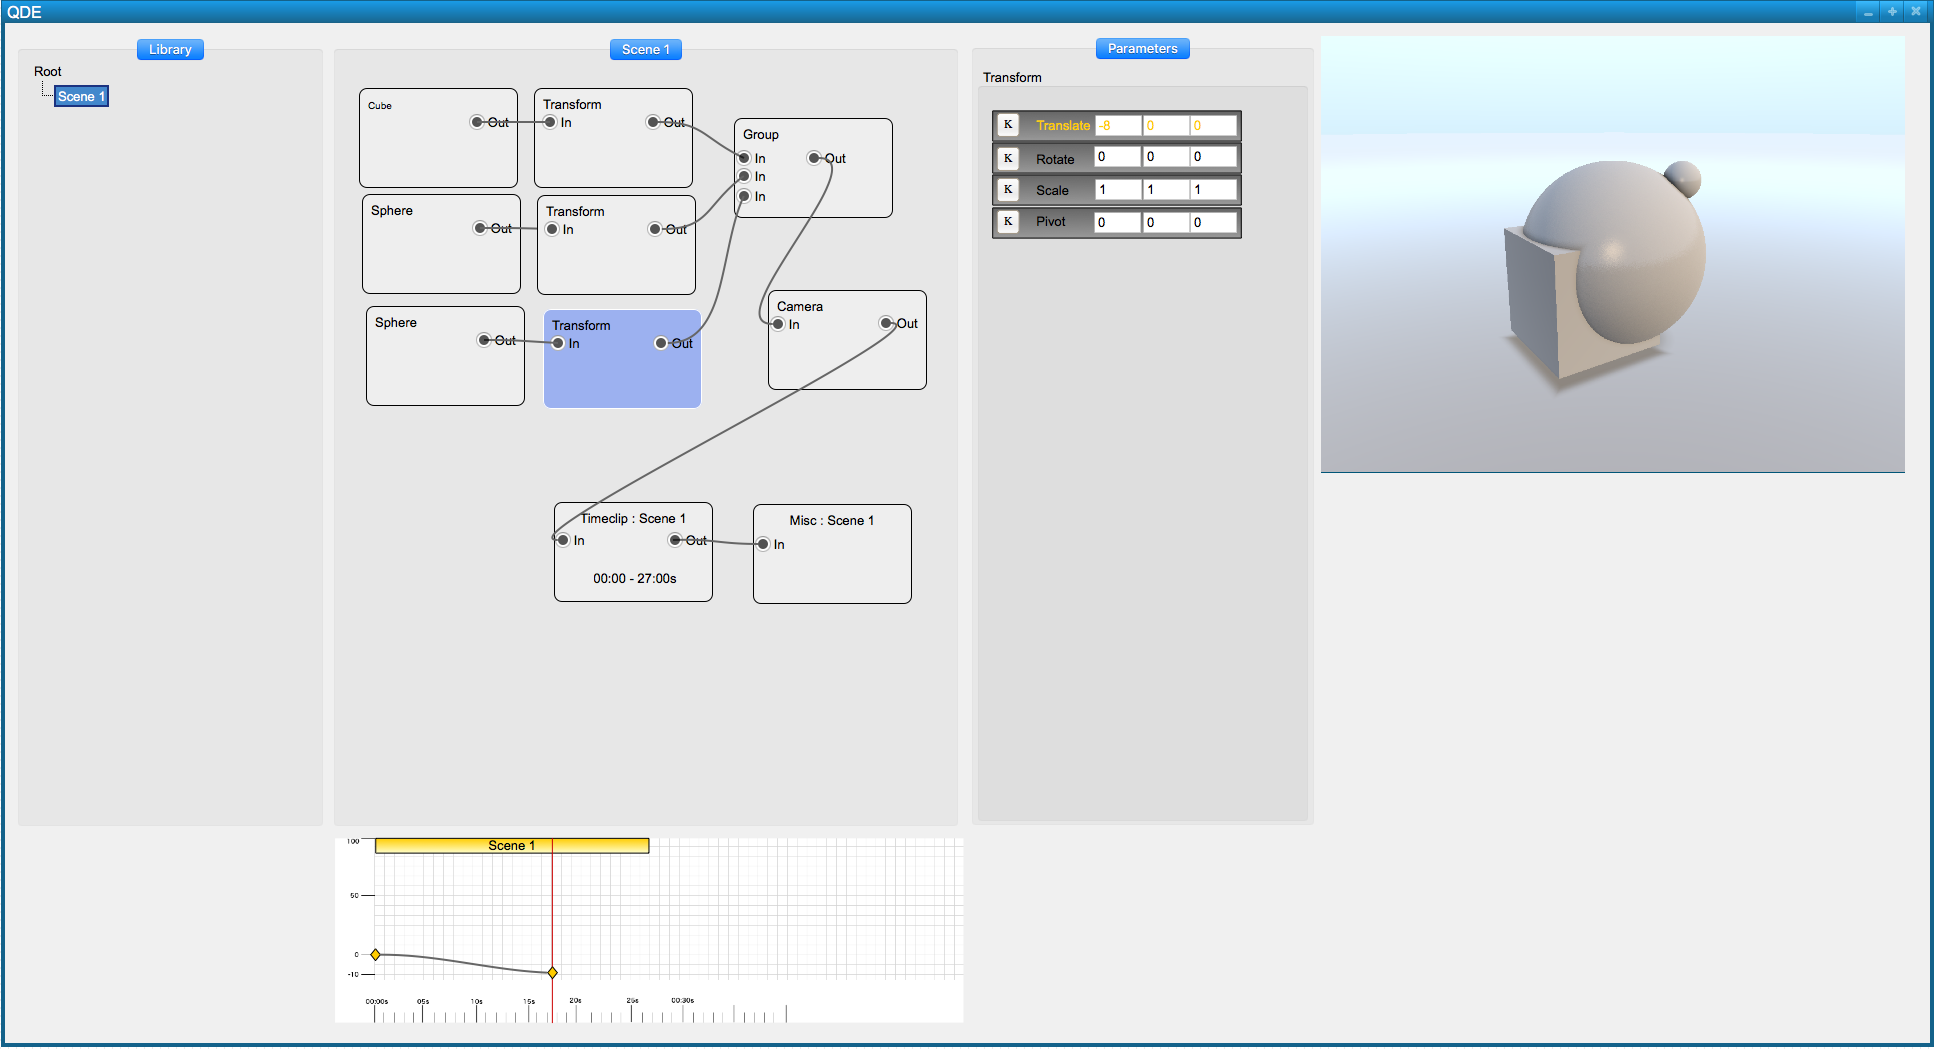
\includegraphics[width=0.9\textwidth]{img/editor_scene1.png}
    \caption{Beispiel-Szene innerhalb des Editors
        \protect\footnotemark}\label{fig:main-components:editor:editor-scene1}
\end{figure}
\footnotetext{Eigene Darstellung mittels Pencil.}

% -*- coding: UTF-8 -*-
% vim: autoindent expandtab tabstop=4 sw=4 sts=4 filetype=tex
% vim: spelllang=de spell
% chktex-file 27 - disable warning about missing include files

\section{Rendering}
\label{sec:prototype:rendering}

Auf das Rendering wird an dieser Stelle nicht näher eingegangen. Ein Teil wird
in~\autoref{sec:prototype:procedure} beschrieben. Der Rest findet sich im
nachfolgenden Kapitel über das verwendete Rendering, siehe~\autoref{chap:rendering}.

